\begin{frame}{Critical Prefix}
    \begin{itemize}
        \item Each interval $\cI$ can be represented as set of \textit{critical prefixes} $\pref_{\cI}$.
        \begin{equation*}
            y \in \cI \quad \leftrightarrow \quad \text{exists prefix } p \prec y, p \in \pref_{\cI}
        \end{equation*}
    \end{itemize}

    \centering
    \begin{tikzpicture}[
        level distance=1.4cm,
        every node/.style={circle,draw,minimum size=6mm},
        level 1/.style={sibling distance=5.6cm},
        level 2/.style={sibling distance=2.8cm},
        level 3/.style={sibling distance=1.4cm,minimum size=5mm},
        marked/.style={fill=green!30,draw=green!60!black}
    ]
        \node (root) {}
            child[edge from parent/.style={draw=none}] { node (nL) {}
                child { node (nLL) {}
                    child { node (l0) {0} }
                    child { node (l1) {1} }
                }
                child { node (nLR) {}
                    child { node[marked] (l2) {2} }
                    child { node[marked] (l3) {3} }
                }
            }
            child[edge from parent/.style={draw=none}] { node (nR) {}
                child { node (nRL) {}
                    child { node[marked] (l4) {4} }
                    child { node[marked] (l5) {5} }
                }
                child { node (nRR) {}
                    child { node[marked] (l6) {6} }
                    child { node (l7) {7} }
                }
            };
        \only<1>{
            \draw[solid] (root) -- (nL);
            \draw[solid] (nL) -- (nLR);
            \draw[solid] (root) -- (nR);
            \draw[solid] (nR) -- (nRL);
            \draw[solid] (nR) -- (nRR);
            \draw[solid] (nRR) -- (l6);
        }
        \only<2>{
            \draw[dashed,thick] (root) -- (nL);
            \draw[dashed,thick] (nL) -- (nLR);
            \draw[dashed,thick] (root) -- (nR);
            \draw[dashed,thick] (nR) -- (nRL);
            \draw[dashed,thick] (nR) -- (nRR);
            \draw[dashed,thick] (nRR) -- (l6);
        }
        \draw[solid] (nL) -- (nLL);
        \draw[solid] (nLL) -- (l0);
        \draw[solid] (nLL) -- (l1);
        \draw[solid] (nLR) -- (l2);
        \draw[solid] (nLR) -- (l3);
        \draw[solid] (nRL) -- (l4);
        \draw[solid] (nRL) -- (l5);
        \draw[solid] (nRR) -- (l7);
    \end{tikzpicture}
\end{frame}